\section{Writing Algorithms in CCP}
\label{sec:ccp}
\begin{table}
    \centering
    \footnotesize
    \begin{tabular}{p{0.35\columnwidth}p{0.5\columnwidth}}
        \hline
        \hline
        \multicolumn{2}{c}{Primitive congestion signals} \\
        \hline
        \hline
        \textbf{Signal} & \textbf{Definition} \\
        \texttt{Ack.bytes\_acked}, \texttt{Ack.packets\_acked} & In-order acknowledged \\
        \texttt{Ack.bytes\_misordered}, \texttt{Ack.packets\_misordered} & Out-of-order acknowledged \\
        \texttt{Ack.ecn\_bytes}, \texttt{Ack.ecn\_packets} & ECN-marked \\
        \texttt{Ack.lost\_pkts\_sample} & Number of lost packets \\
        \texttt{Ack.now} & Datapath time (e.g., Linux \texttt{jiffies})\\
        \texttt{Flow.was\_timeout} & Did a timeout occur? \\
        \texttt{Flow.rtt\_sample\_us} & A recent sample RTT \\
        \texttt{Flow.rate\_outgoing} & Outgoing sending rate \\
        \texttt{Flow.rate\_incoming} & Receiver-side receiving rate  \\
        \texttt{Flow.bytes\_in\_flight}, \texttt{Flow.packets\_in\_flight} & Sent but not yet acknowledged \\
        & \\
        \hline
        \hline
        \multicolumn{2}{c}{Operators} \\
        \hline
        \hline
        \textbf{Class} & \textbf{Operations} \\
        Arithmetic & $+, -, *,$~/$,$ EWMA \\
        Assignment & $:=$ \\
        Comparison & $==, <, >$, or, and \\
        Conditionals & If (branching) \\
        & \\
        \hline
        \hline
        \multicolumn{2}{c}{Variable Scopes} \\
        \hline
        \hline
        \textbf{Scope} & \textbf{Description} \\
        \texttt{Ack} & Signals measured per packet \\
        \texttt{Flow} & Signals measured per connection \\
        %% \texttt{Control} & Never reset except by \texttt{update\_fields()} in user-space \\
        %% \texttt{Report} & Maintained until a call to \texttt{(report)}, then reset to defaults \\
        \texttt{Timer} & Multi-resolution timer that can be zeroed by a call to \ct{reset} \\
    \end{tabular}
    %\vspace{0.075in}
    \caption{Fast path language: primitive signals, operators, and scopes.}\label{tab:api}
\end{table}

Writing an algorithm in CCP involves two considerations: logic in CCP and in the datapath.
This ``split'' programming model involving both a slow and a fast execution environment allows
algorithms to perform computations flexibly in CCP, \eg compute a cubic
root or use a machine learning algorithm to determine a sending rate, while
providing high performance by retaining frequently invoked logic within
the datapath.

Implementing the CCP portion of an algorithm involves writing two callback methods:
\ct{onCreate()} and \ct{onReport()}.
In turn, the \texttt{onCreate()} function should install an
event-driven program in the fast path.
Programs running in the datapath could compute summaries over per-packet
information (such as a minimum packet delay or a moving average of packet
delivery rate) and explicitly report summaries or high priority conditions
(such as loss) to CCP.
On a report, CCP calls the \ct{onReport()} handler,
allowing the congestion control algorithm to set the flow's congestion
window or sending rate, or replace the datapath program with different logic.

\paragrapha{Datapath programs} CCP's datapath programs are written in a restrictive
domain-specific language.
Conceptually, datapath programs contain state initializations, \ie a \ct{def}
clause, and event specifications, \ie a series of \ct{when} clauses.
The fast path checks event conditions on every incoming packet and timeout event.
If an event condition evaluates to true, the body of the \ct{when} clause is executed as the corresponding
action.
For example, the following program counts the cumulative
number of packets acknowledged and lost, and it reports these counters immediately upon a loss:

{\footnotesize
\begin{minted}{lisp}
(def (Report (volatile acked 0) (volatile lost 0)))
(when true
  (:= Report.acked (+ Report.acked Ack.bytes_acked))
  (:= Report.lost  (+ Report.lost  Ack.lost_pkts_sample))
  (fallthrough))
(when (> Report.lost 0) (report))
\end{minted}
}

Here, \texttt{(when true ...)} signifies that the body should be evaluated on every packet.
Correspondingly, \texttt{(fallthrough)} indicates that subsequent \texttt{when} clauses should be evaluated.
The \ct{report} instruction causes the datapath to
transmit the \ct{acked} and \ct{lost} byte counters to the slow path whenever
the \ct{lost} counter becomes greater than zero.
Since \ct{acked} and \ct{lost} are marked \ct{volatile}, these values are reset to their initial value, 0, 
after every call to \ct{report}.

Fast path programs have read access to {\em primitive congestion signals} 
(prefixed with ``\ct{Ack.}'' or ``\ct{Flow.}'' to specify their measurement period) that are
exposed by the kernel on every incoming packet.
Such signals include statistics such as the round trip delay sample obtained
from the packet, the number of bytes that the stack believes have been dropped
by the network, the delivery rate of packets at the receiver, and so on.
Table~\ref{tab:api} enumerates the primitive congestion signals we support.

\paragrapha{CCP Algorithm Logic} The \ct{onReport()} handler provides a way to
implement congestion control actions in \userspace in reaction to reports from the datapath.
For example, a simple additive-increase
multiplicative-decrease (AIMD) algorithm could be implemented in Python\footnote{Our CCP implementation is in Rust and exposes Python bindings.} using
the \ct{acked} and \ct{lost} bytes reported every round-trip time from the datapath:

{\footnotesize
\begin{minted}{python}
def onReport(self, report):
  if report["lost"] > 0:
     self.cwnd = self.cwnd / 2
  else:
     acked = report["acked"]
     self.cwnd = self.cwnd + acked*MSS/self.cwnd
  self.update("cwnd", self.cwnd/MSS)
\end{minted}
}

We have implemented complex functionality within congestion control algorithms
by leveraging slow-path logic, for example, a congestion control
algorithm that uses signal processing techniques~\cite{nimbus}.

If the round-trip time of the network is a few milliseconds or more,
it is possible to locate congestion control algorithm logic entirely within CCP
with high fidelity relative to a per-packet update algorithm, as we show in \S\ref{sec:eval:fidelity}.

\subsection{Example: BBR}
\label{s:ccp:bbr}
As a more involved example, we show below
how various components of TCP BBR~\cite{bbr} are implemented using the CCP API.
A BBR sender estimates the rate of packets delivered to the receiver, and sets
its sending rate to the maximum delivered rate (over a sliding time
window), which is believed to the rate of the bottleneck link between the sender
and the receiver.

This filter over the received rate is expressed simply in a fold function:
{\footnotesize
\begin{minted}{lisp}
(when true
    (:= minrtt (min minrtt Ack.rtt_sample_us))
    (:= curr_btl_est (max curr_btl_est Flow.rate_incoming))
    (fallthrough))
\end{minted}
}

To determine whether a connection can send more than its current sending rate,
BBR probes for additional available bandwidth by temporarily increasing its
sending rate by a factor (1.25$\times$) of its current sending rate.
%
To drain a queue that may have been created in the process, it also reduces its
rate by a reciprocal factor (0.75$\times$) before starting to send at the new estimated
bottleneck link rate.

The following excerpt expresses this sending pattern (for simplicity, we show only 2 transitions):
{\footnotesize
\begin{minted}{lisp}
(when (== pulseState 0)
  (:= Rate (* 1.25 curr_btl_est))
  (:= pulseState 1))
(when (&& (== pulseState 1) 
          (> Timer.micros Flow.rtt_sample_us))
  (:= Rate (* 0.75 curr_btl_est))
  (:= pulseState 2))
\end{minted}
}

Here, the variable \ct{pulseState} denotes the state of the sender's
bandwidth probing: probing with high sending rate (0) and draining queues with low
sending rate (1).
Each \texttt{when} clause represents a pulse state transition and is conditioned on the
resettable timer \texttt{Timer.micros}.
Upon the transition, the handler sets the \texttt{Rate} and advances \texttt{pulseState}.
After the last phase of the pulse, the handler would reset the timer and \ct{pulseState} to restart the sending pattern (not shown).

Figure~\ref{fig:ccp:bbr} shows\footnote{We only implement BBR's bandwidth and RTT probing (PROBE\_BW and PROBE\_RTT) phases. Our implementation is here: \an{link to CCP BBR implementation}.}
the impact of BBR's bandwidth probing on the
achieved goodput and queueing delays when a single flow runs over a 96 Mbit/s
bottleneck link with a 100 ms round trip propagation delay.
%
BBR's windowed min/max operations and the RTT probing phase (showing steep rate
dips every 10 seconds) are implemented in the slow path's \ct{onReport()}
handler by installing a new fold function.
%
CCP's split programming model enables such flexible partitioning of
functionality, whereby complex operations and special cases can be implemented
in \userspace.

\begin{figure}[t]
\centering
    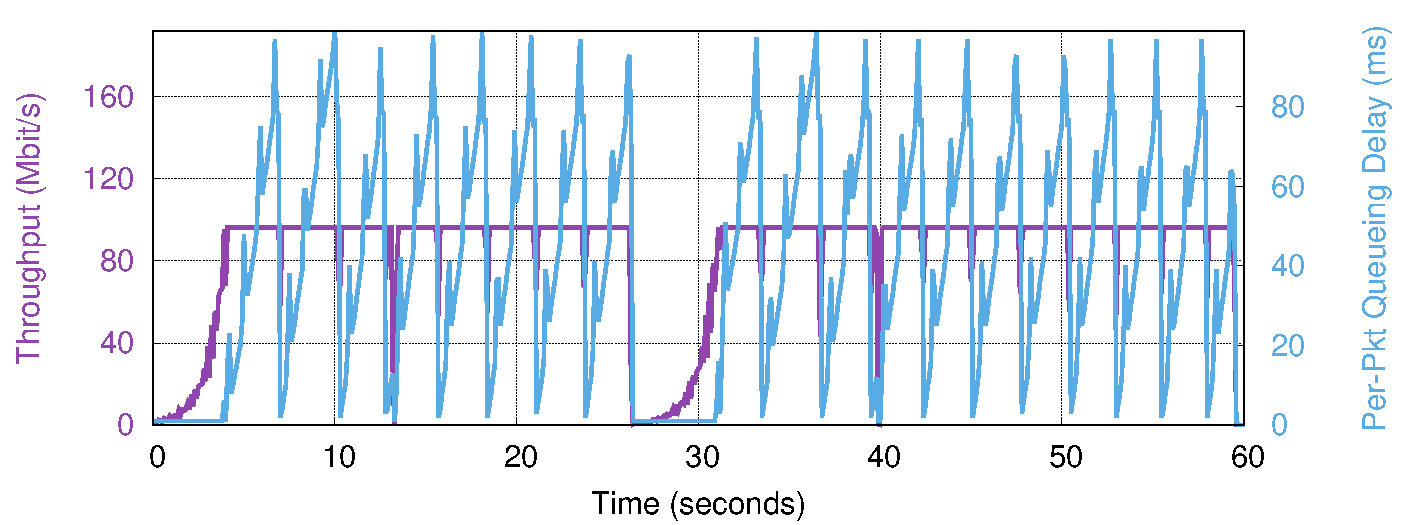
\includegraphics[width=\columnwidth]{img/bbr}
    \caption{
    Our CCP implementation of BBR used for a bulk transfer over a 96 Mbit/s link with a 100 ms RTT. The bandwidth probe phase can be seen in the oscillation of the queueing delay, and the RTT probe phase can be seen in the periodic dips in throughput.
    }\label{fig:ccp:bbr}
\end{figure}

\subsection{Case Study: Slow Start}
\label{s:ccp:ss}

Because algorithms no longer make decisions upon every ACK, CCP changes the way in which developers should think about congestion control, and correspondingly provides multiple implementation choices. As a result, new issues arise about where to place algorithm functionality. We discuss the involved trade-offs with an illustrative example: slow start.

Slow start is a widely used congestion control module in which a connection probes for bandwidth by multiplicately increasing its congestion window (\texttt{cwnd}) every RTT. Most implementations increment \texttt{cwnd} per ACK, either by the number of bytes acknowledged in the ACK, or by 1 MSS. With CCP, one way to implement slow start is to retain the logic entirely in CCP, and measure the size of the required window update from datapath reports. We show an example in Listing~\ref{lst:ccp:ss}. This implementation strategy is semantically closest in behavior to native datapath implementations.

\begin{listing}[t]
{\footnotesize
\begin{minted}{rust}
fn create(...) {
  datapath.install("
  (def (Report (volatile acked 0) (volatile loss 0)))
  (when true 
    (:= Report.acked (+ Report.acked Ack.bytes_acked)))
  (when (> Micros Flow.rtt_sample_us) (report) (reset))");
}
fn onReport(...) {
  let acked = report.get_field("Report.acked");
  self.cwnd += acked;
  datapath.update_field(&[("Cwnd", self.cwnd)]);
}
\end{minted}
}
\caption{A CCP implementation of slow start (exiting slow start not shown).} \label{lst:ccp:ss}
\end{listing}

\begin{figure}
    \centering
    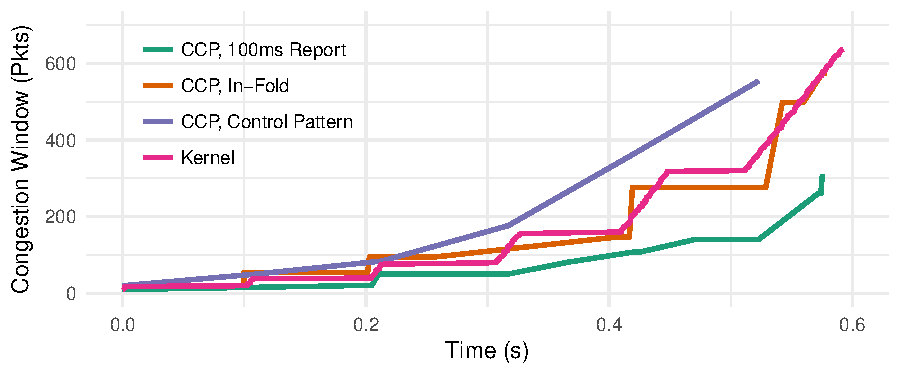
\includegraphics[width=\columnwidth]{img/ss-evo}
    \caption{Different implementations of slow start have different window update characteristics. The control pattern implementation is rate-based, so we show the congestion window corresponding to the achieved throughput over each RTT.}
    \label{fig:ccp:ss}
\end{figure}

For some workloads this approach may prove problematic, depending on the parameters of the algorithm. If the reporting period defined is large, then infrequent slow start updates can cause connections to lose throughput.
Figure~\ref{fig:ccp:ss} demonstrates that, on a $48$ Mbps, $100$ ms RTT link, different implementations of slow start exhibit differing window updates relative to the Linux kernel baseline.
An implementation with a 1-RTT reporting period lags behind the kernel, but it is also possible to implement slow start within the datapath (Listing~\ref{lst:ccp:ssfold}), or using the control pattern style: 

{\footnotesize
\begin{minted}{lisp}
(when (> Timer.Micros Flow.rtt_sample_us)
    (:= Rate (* Rate 2))
    (:= Timer.Micros 0))
\end{minted}
}

\paragrapha{Take-away} As outlined in \S\ref{s:design}, the programming model of fold functions is deliberately limited.
First, we envision that in the future, CCP will support low-level hardware datapaths---the simpler the fold function execution environment is, the easier these hardware implementations will be. Second, algorithms able to make complex decisions on longer time-scales will naturally do so to preserve cycles for the application and datapath; as a result, complex logic inside the fold function may not be desirable.

More broadly, developers may choose among various points in the algorithm design space. 
On one extreme, algorithms may be implemented almost entirely in CCP, using the fold function as a simple measurement query language.
On the other extreme, CCP algorithms may merely specify transitions between in-datapath fold functions implementing the primary control logic of the algorithm.
Ultimately, users are able to choose the algorithm implementation best suited to their congestion control logic and application needs.

\begin{listing}[t]
{\footnotesize
\begin{minted}{rust}
fn create(...) {
  datapath.install("
  (def (volatile Report.loss 0))
  (when true (:= Cwnd (+ Cwnd Ack.bytes_acked)))
  (when (> Ack.lost_pkts_sample 0) (report))");
}
fn onReport(...) {
  // exit slow start
}
\end{minted}
}
\caption{A within-fold implementation of slow start. Note that CCP algorithm code is not invoked at all until the connection experiences its first loss.} \label{lst:ccp:ssfold}
\end{listing}
